\documentclass[12pt]{article}
\usepackage{amsfonts, epsfig}
\usepackage[authoryear]{natbib}
\usepackage{graphicx}
\usepackage{fancyhdr}
\pagestyle{fancy}
\lfoot{\texttt{comsm0094.github.io}} \lhead{LC\&B - 01.6 Recording from the brain - Conor} \rhead{\thepage} \cfoot{}
\begin{document}

\section*{Recording from the brain}

In the earliest days of philosophy and science there was a belief that
we could make progress in understanding the brain by thinking about
thought, by a complex process of structured introspection. It is
likely that this still has a role in our broad subject, but it is
equally clear that the fact of science, the facts we can discover by
observing the dynamics of neural matter, are vital to understanding
the brain. The tools of neuroscience were for a long time very crude;
as we saw, the main approach was to study patients while they were
alive and then dissect them after they died. Now, though, we have a
diversity of approaches to recording the dynamics of neural matter.

The ideal, obviously, would be to record all the voltage changes for
all the neurons in the brain and, probably, the different levels of
different chemical. That isn't possible and any approach to recording
from the brain is a compromise between spatial and temporal resolution
and between the degree of intervention: at one extreme \textsl{in
  vitro} experiments are done on slices of brain that have been
removed from an animal, typically one that has been killed as part of
the experiment, these experiments can record the voltage inside the
neuron an sub-milisecond resolutions. At the other extreme
\textsl{electroencephalography} is completely non-invasive, you might
end up with conductive gel on your hair but beyond that, there is no
ill-effect or annoyance to the subject, but the date is very noisy and
is a sort of smeared out average of the activity of lots of synapses.

This document is intended only as a quick tour of some recording
techniques: the speed at which the field is advancing and the vast
diversity of approaches means any description is only very partial and
slightly out-of-date. I will only mention ways of recording brain
activity, but this has been paralleled by technologies to distinguish
different cells, for example, using dyes that transport backwards
through a synapse allowing researches to see what cell is connented to
which and technologies, such as optogenetics and Designer Receptors
Exclusively Activated by Designer Drugs (DREADDs), which can switch on
or off specific cell populations, allowing researchers to work out
what different cells are contributing to network activity.

\subsection*{In vitro electrophysiology}

In \textsl{in vitro} electrophysiology a small piece of the brain is
removed and placed in a dish where it is kept alive by careful control
of chemical composition and oxygen level of the fluid the slice is
bathed in. An electrode is then used to record from the cell; this
electrode is often a thin glass tube filled with salty water and it
sort of ``sucks'' onto the cell making a seal, see
Fig.~\ref{fig:patch}. This approach typically gives a complete
recording of the voltage inside in the cell; it can be used, for
example, to measure the size of an PSP, the dendritic voltage change
at a synapse.

Slices are usually made in a way that preserves as much of the
neurites, the axons and dendrites, as possible; this is easier in some
parts of the brain than others, the hippocampus for example lends
itself to \textsl{in vitro} approaches because it has a very laminar
structure and a lot of what we know about synapses was discovered in
hippocampus. However, the key point is that these neurons are not in
their natural environment, they will have damaged neurites, the
chemical and temperature environment is not normal and their input is
nothing like what it would be in the brain.

\begin{figure}
  \begin{center}
    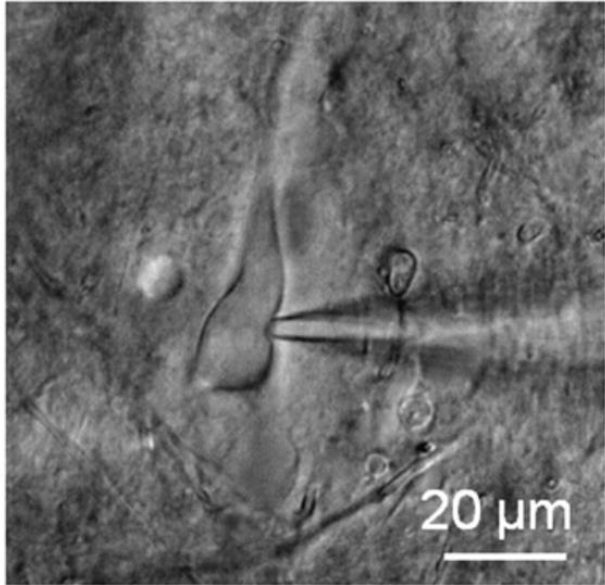
\includegraphics[width=6cm]{patch.png}
    \end{center}
  \caption{\textbf{Patched cell}: here an electrode has been \textsl{patched clamped} onto a cell to record its internal voltage. [figure from Ding, S., Mattam, S. G. \& Zhou F. M. (2011)]\label{fig:patch}}
\end{figure}

One nice approach, which has been used a lot in studying the retina,
is to lay the slice directly only an array of electrodes. This does
not give \textsl{intracellular data}: the electrodes record from
outside the cell, giving \textsl{extracellular data}, so the data are
spike times rather than voltages, but the density of electrodes that
are possible does give a very complete picture of the network
activity, albeit in this weird context.

\subsection*{In vivo electrophysiology}

The \textsl{vitro} in \textsl{in vitro} means glass, referring I think
to the glass dish the brain slice is placed in. In contrast, the
\textsl{vivo} in \textsl{in vivo} means living and \textsl{in vivo}
electrophysiology is performed using living animals, either
anesthetized or awake and behaving. To do this an electrode is placed
in the animals brain; in the anesthetized preparation a hole is cut in
the brain, \textsl{trepanation}, and the electrode is inserted through
that, or, in the awake behaving preparation, a \textsl{head stage} is
mounted on the head covering and sealing up a hole in the skull. In
the past the electrode was moved until the activity it recorded showed
it was near a neuron; these days though silicon probes can be
used. Silicon probes are made using processes similar to those used to
manufacture chips and have hundreds of recording sites; in this case
the experimenter will rely on at least some of the recording sites
being near the neurons.

In an \textsl{in vivo} experiment the electrode is outside the neuron
so only the spikes are recorded and typically, spikes from more than
one neuron are mixed together. A set of algorithms called
\textsl{spike sorting} are used to assign spikes to different
neurons. The accuracy of spike sorting is often debated; with silicon
probes spikes are often recorded, with different amplitudes, by
different recording sites, something that was already possible, but in
a much more limited way, with simpler electrodes; this allows a sort
of triangulation to be performed in spike sorting, making it more
accurate for silicon probes, however, the amount of sorting involved
with silicon probes, given their vast number of recording sites, means
the debate about how to best spike sort is as heated as ever.

The advantage of \textsl{in vivo} electrophysiology is that you can
record from the brain in a more natural state; however, the need to
tether the electrode to the recording equipment in the awake behaving
preparation limits the experiments that can be performed. Furthermore,
the data recorded gives spikes, not voltages and spiking activity
rather than synaptic activity. Although the number of neurons that can
be recorded has increased a huge amount over the last few years, it is
still a long way from recording whole brain activity. It can also be
difficult to decide exactly what sort of neuron you are recording
from, although different cells have different firing properties they
are not always distinct enough to be distinguishable from their spike
trains. It is a highly invasive procedure, there are animal welfare
concerns and, except in very limited circumstances related to medical
treatment, it is not possible to record from humans. Nonetheless
\textsl{in vivo} electrophysiology has been one of the main tool of
neuroscience over the last 50 years and has been the source a lot of
the progress that has been made, see as just one example
Fig.~\ref{fig:place}


\begin{figure}
  \begin{center}
    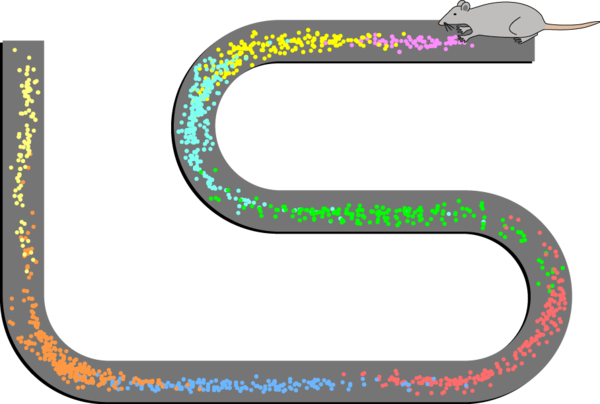
\includegraphics[width=8cm]{place_cells.png}
    \end{center}
  \caption{\textbf{Place cells}. Here each color of dot corresponds to a different neuron and the dots are placed on the maze in the location the rat was in when a spike in one of the eight neurons was fired. It shows clear evidence of place cells, with different cells firing in different locations. [figure from wikipedia]\label{fig:place}}
\end{figure}

\subsection*{Calcium imaging}

Although, for simplicity and for historical reasons, the story we tell
about neuronal dynamics focuses on the movement of sodium and
potassium ions, in fact, in mammalian brains calcium ions play a big
role in spiking, in synaptic signalling and in plasticity. Over the
last few years it has become possible using either genetic animals or
special dyes to introduce into brain cells, in living animals,
chemicals that bond with calcium and emit photons. This really is
incredible; it is also very useful, using two-photon microscopy it is
possible to measure the voltage of neurons. This allows a large number
of neurons to be imaged and recorded and, often, allows the same cells
to be recorded from over a long period or even across successive days;
since the recording is linked to an image, it is often possible to
identify cell type and to study development. Huge numbers of neurons
can be recorded.

Obviously there are many constraints on calcium imaging. For a start,
the dynamics of the dye are slower than the dynamics that produces
spikes, so complicated \textsl{deconvolution} algorithms are needed to
deduce spike times from luminescence. In addition, and more obviously,
the experiment needs a window into the brain and a large microscope
pointing at it. This rules out straight-forward awake behaving
experiments, instead typically experiments use a \textsl{head-fixed}
preparation. For a rodent, the head of animal stands on a wheel or
ball, free to move, but with its head fixed under the microscope and
with a monitor in front of it: of this is rather grandly called a
virtual reality experiment, but that amounts to little more than
linking the picture on the monitor to the movement of the wheel or
ball. Another, very impressive, example, involves the developing
zebrafish, hatchling zerbafish respond to optical flow, the movement,
or apparent movement, of the river bed. Since hatching zebrafish are
transparent, a huge fraction of its neurons can be recorded at once.

The glory of calcium imaging is that you can see the activity of
neurons spread across the piece of the brain that is being imaged, so
rather than including an image here I urge you to go and look at
videos on youtube.

\subsection*{Electroencephalography}

In electroencephalography (EEG) electrodes are placed on the scalp,
usually of human participants and these are used to record the
electrically activity in the brain. The story behind the discovery of
EEG is amusing, you can read about it by looking up Hans Berger on
wikipedia; in short, he wanted to explain what he believed was the
real phenomena of telepathy. It is surprising that EEG works, the
biggest electrically signals in the brain come from the activity in
synapses, if all the synapses were in random directions these signals
would all cancel out; it turns out that, particularly in cortex, there
is some bias in the orientation in synapses, leading to an overall
electrical field that can be measured at the scalp.

Needless to say, EEG signals are incredibly noisy, they mix together a
plethora of neural activity and average a huge number of tiny
electrical fields. The spatial resolution is terrible. However, the
key advantage of EEG is two fold, it has good temporal resolution and
it is easy to do, it is non-invasive, portable and relatively
inexpensive. It was, for a long time, an important diagnostic tool;
when I had childhood migraine for example, I was given an EEG; these
days I would probably have an MRI. It has been of considerable help in
studying epilepsy and lead to the discovery of sleep stages, the
distinction between slow wave and REM sleep. I use EEG data in my own
work on language since linguistic processing happens at short temporal
scales and the only useful experimental subjects are humans. There is
an example EEG trace, from a medical case report, in
Fig.~\ref{fig:eeg}.

Magnetoencephalography (MEG), which detects magnetic fields rather
than electrical ones produces better data, basically the magnetic
fields aren't screened in the same way by the brain fluid; but MEG is
much more expensive, the instruments used to measure magnetic field
require superconductors and, thus, need to be cooled. There is
optimism that a new technology, optically-pumped magnetometry, will
lead to a cheaper and less cumbersome version of MEG.



\begin{figure}
  \begin{center}
    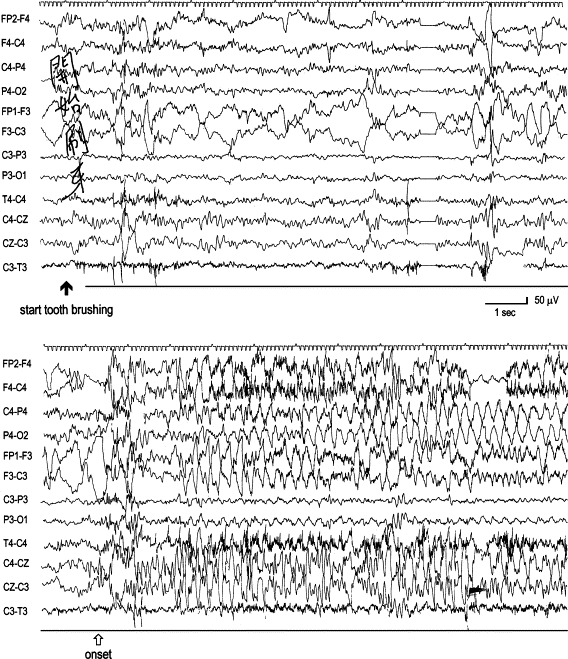
\includegraphics[width=8cm]{eeg.png}
    \end{center}
  \caption{\textbf{EEG}. This shows the EEG traces from a woman who
    has epileptic fits, accompanied by orgasm, when she bushes her
    teach; the moment she starts toothbrushing are marked by arrows
    and the over-synchonized activity typical of epilepsy is seen soon
    afterwards. [figure from Chuang, Yao-Chung, et al. "Tooth-brushing
      epilepsy with ictal orgasms." Seizure 13.3 (2004):
      179-182.]\label{fig:eeg}}
\end{figure}



\subsection*{Magnetic resonance imaging}

In magnetic resonance imaging (MRI) an oscillating magnetic field is
used to shift atoms between different energy states, this causes them
to release radio-frequency electro-magnetic radiation, which can in
turn be detected. By changing the oscillations, different sorts of
things can be imaged; a structural scan can be used to get a very
detailed image of the brain. This is very important in diagnostics,
the brain can't be x-rayed; since neural matter has the same density
as the fluid around it, by design of course to protect the brain, it
is invisible in x-rays. As recently as the 70s the only way to image
the brain if a tumour was suspected was to introduce an air bubble
into the skull and then x-ray the brain while trying by head movements
to get the bubble in the right place. Another type of scan,
tensor-diffusion imaging, is able to find neural tracts, showing how the brain is connected, see Fig.~\ref{fig:dti}.


\begin{figure}
  \begin{center}
    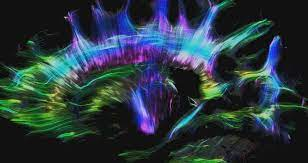
\includegraphics[width=8cm]{dti.jpeg}
    \end{center}
  \caption{\textbf{Diffusion tensor imaging}. DTI allows us to image the connectivity of the brain. [figure from wikipedia.]\label{fig:dti}}
\end{figure}

For our purposes, the most important type of MRI is functional MRI. In
fMRI the oscillations are tuned to excite oxygen, giving what is
called the BOLD signal, a measure of the level of oxygenated blood in
a part of the brain. This is believed to track activity, so fMRI can
show which parts of the brain are active while the participant
performs a task: the task of course being constrained by the MRI
machine itself, the MRI machine is a huge cylinder with the subject,
or patient, slotted into a hole at its centre; if you've never had an
MRI the machine will be familiar to you from TV where it is often used
as a short hand for `serious medical stuff', see
Fig.~\ref{fig:mri}. The fMRI images have poor temporal resolution,
basically the bold signal is giving the average activity of the brain
over about three seconds; the spatial resolution, however, is pretty
good; each voxel, the area resolved by the machine, is a cubic
milimeter.


\begin{figure}
  \begin{center}
    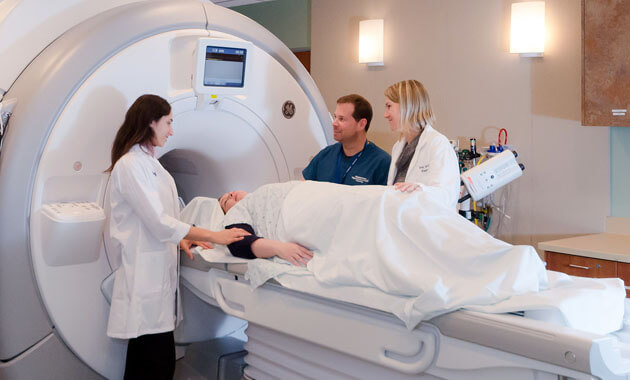
\includegraphics[width=8cm]{mri.jpg}
    \end{center}
  \caption{\textbf{MRI machine}. A patient about to enter an MRI
    machine; the experience is a little claustrophic and very noisy,
    the magnets make a noise, but not unpleasant. [figure from
      radiology.ucsf.edu.]\label{fig:mri}}
\end{figure}



\begin{figure}
  \begin{center}
    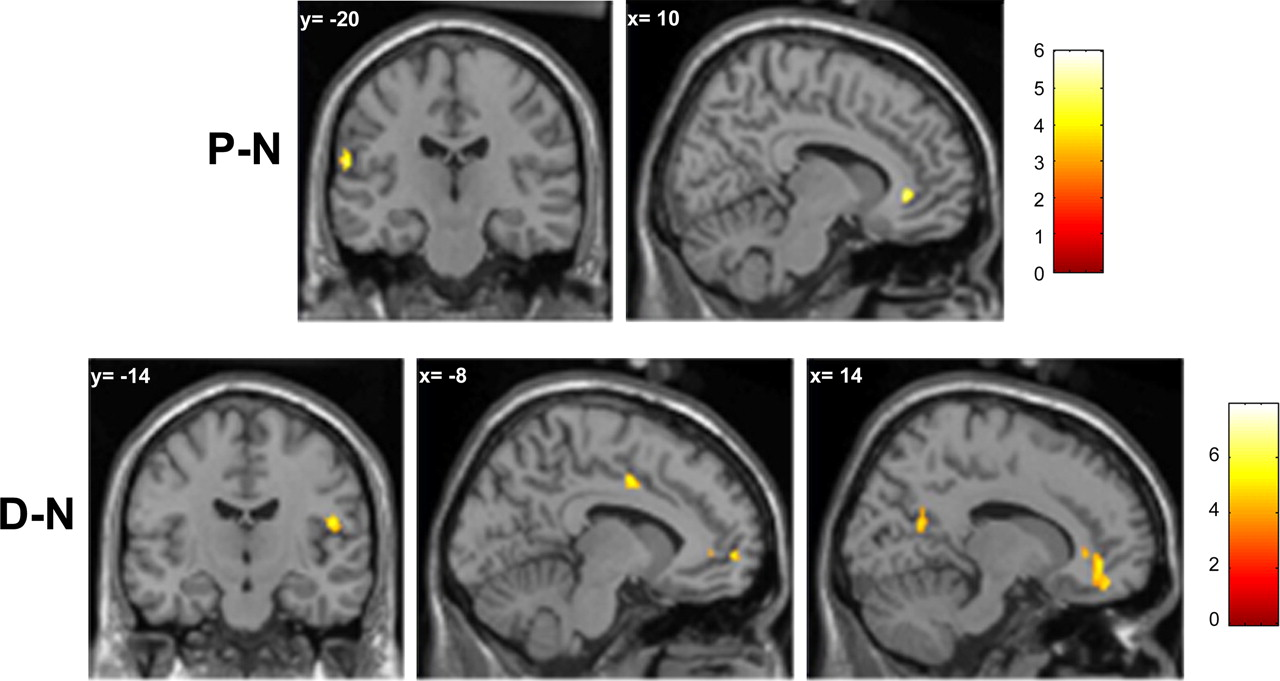
\includegraphics[width=8cm]{fmri.jpg}
    \end{center}
  \caption{\textbf{fMRI images}. An fMRI study to distinguish the parts of the brian responding to disgusting or painful looking images [figure from Benuzzi, Francesca et al. Does It Look Painful or Disgusting? Ask Your Parietal and Cingulate Cortex, Journal of Neuroscience, 28 923-931]\label{fig:mri}}
\end{figure}

\subsection*{Summary}
All approaches to recording from the brain are a trade-off between how
much of the brain is recorded, how good the resolution is, how
invasive it is, how much it constrains any behaviour and how much it
costs. \textsl{in vitro} physiology measures in the voltage inside the
cell, but only for brain slices, \textsl{in vivo} electrophysiology
measures spikes in the living brain, often in awake and behaving
animals, the number of cells that can be recorded from is limited but
increasing. Calcium imaging records from a huge number of cells, but
the experiments are difficult and the behaviour constrained. EEG and
fMRI experiments can be used with human participants, the first has
poor spatial resolution, the second poor temporal resolution and both
are a long long way from recording from individual neurons.




\end{document}

